\documentclass[utf8, 11pt]{feuille}

\newcommand{\titredutd}{\textbf{CC2 --- Ensembles canonique et grand-canonique}}

\begin{document}

\begin{center}
    \Large {\bf Contrôle continu}
    
    Mercredi 10 novembre 2021 - durée: 2h00
\end{center}

Seules les calculatrices non communicantes et les notes manuscrites personnelles sont autorisées.

Les exercices sont totalement indépendants.

%\begin{tcolorbox}[
        colback=gray!20,
        colframe=gray!20,
        width=\dimexpr\textwidth\relax, 
        arc=0pt,outer arc=0pt,
        ]

\texttt{Seules les calculatrices non communicantes et les notes manuscrites personnelles sont autorisées.}

\texttt{Les exercices sont totalement indépendants.}

\texttt{On notera $k_B$ la constante de Boltzmann et $h$ la constante de Planck.}

\end{tcolorbox}



% ______________________________________________________________________________


\section{Une balance ultrasensible}

On accroche une masse $m$ à une balance très sensible constituée par un ressort sans masse de raideur $\alpha$. L'ensemble est à l'équilibre thermique avec une enceinte à la température $T$. On désigne par $g$ l'accélération de la pesanteur et on introduit $\omega^2=\frac{\alpha}{m}$. On suppose que le seul degré de liberté du système masse-ressort est la position selon la verticale de la masse. L'hamiltonien  s'écrit alors ${\cal H}=\frac{p_z^2}{2m}+mgz+\frac{1}{2} m\omega^2 z^2$.

\medskip

\question Donner le sens des différents termes de l'hamiltonien. \`A quel choix de l'origine ($z=0$) correspond cet hamiltonien ? 

\question Calculer la fonction de partition $Z$ du système. Sous quelles conditions peut-on considérer que $-\infty < z < +\infty$ ? On rappelle que $\int_{-\infty}^{+\infty} \exp(-u^2) du= \sqrt{\pi}$. Montrer par un changement de variable approprié que $Z=\frac{1}{\beta \hbar \omega} \exp(\frac{\beta m g ^2}{2 \omega^2})$

\question Relier la valeur moyenne $\overline z$ de la position à une dérivée partielle de $\ln Z$ par rapport à une variable judicieusement choisie. Faire de même avec $\sigma^2=\overline{z^2} - \overline{z}^2$   et une dérivée partielle seconde de  $\ln Z$.

\question Calculer $\overline z$. Ce résultat était-il prévisible ? Calculer $\sigma^2$. Quelle est l'origine physique des fluctuations de la position de la masse ?

\question Pensez vous que l'on puisse construire un ressort permettant de mesurer la constante de Boltzmann à partir de la mesure des fluctuations de position ? On justifiera sa réponse en donnant des ordres de grandeurs.

\section{ Élasticité de la laine}
On peut modéliser la laine par une longue chaîne de $N \gg 1$ molécules identiques, que l'on suppose discernables et indépendantes les unes des autres. Une telle chaîne est appelée macromolécule ou polymère. Chaque molécule (ou monomère) peut se trouver
dans deux états notés $1$ et $2$ (voir figure). Dans l’état $1$, la molécule contribue pour $a$ à la longueur de la
chaîne et son énergie est $\epsilon_{a}$. Dans l’état $2$, sa longueur est $b$ et son énergie $\epsilon_{b}$. La chaîne est
soumise à une tension $F$ et est en équilibre avec un thermostat à la température $T$. L'énergie de la chaîne s'écrit dans ces conditions $E=\sum_{i=1}^{N} \epsilon_i-F\sum_{i=1}^{N} l_i$ où $l_i=a$ ou $b$ et $\epsilon_i=\epsilon_{a}$ ou $\epsilon_{b}$ selon la conformation $1$ ou $2$ du monomère $i$. {\bf On notera que $\bf a > b$}. Pour le calcul des ordres de
grandeur, on prendra $a = 2b = 2$ nm et $N = 10^4$.

\ 

\centerline{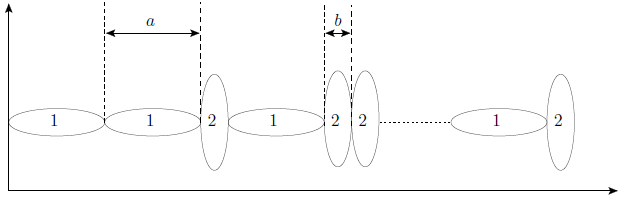
\includegraphics[height=.17\textwidth]{keratine.png}}

\question Calculer la fonction de partition de la chaîne. 

\question En déduire son énergie moyenne $\overline{E}$ et sa longueur moyenne $\overline{L}$ à l'équilibre en fonction de $F$ et $T$.

On se place maintenant dans l'approximation où $\epsilon_{a} \approx \epsilon_{b}$.

\question Simplifier les expressions obtenues dans les questions ci-dessus.

\question \'Etudier, pour $F$ donnée, les limites basse température et haute température  de $\overline{E}$ et de $\overline{L}$. Interpréter les résultats.

\question Donner l'allure de la courbe $\overline{l}=\frac{\overline{L}}{N}$ en fonction de $F$ à $T$ donnée. Comment dans le cas des grandes forces $\beta F (a-b) \gg 1$, la limite asymptotique est-elle approchée ?

\question Montrer que dans le domaine des faibles forces, la chaîne vérifie la loi $F=K(T) (\overline{L} - L_0)$. Déterminer et interprétér $K(T)$ et $L_0$. Comment s'appelle cette loi ? Donner l'ordre de grandeur à température ambiante pour ces deux paramètres.

\question Peut-on en conclure quelque chose sur le lavage de la laine ?

\section{Empoisonnement par le \st{dioxyde} monoxyde de carbone }

Lorsqu'il y a empoisonnement par le monoxyde de carbone, les molécules de $CO$ remplacent les molécules d'$O_2$, adsorbées sur les molécules d'hémoglobine ($Hb$) du sang. Pour montrer cet effet, on considère un modèle dans lequel chaque site des molécules $Hb$ peut être vacant avec une énergie nulle, ou occupé, soit par une molécule $O_2$ avec l'énergie $E_A$, soit par une molécule de $CO$ avec une énergie $E_B$. L'occupation d'un site n'a aucune influence sur l'occupation des autres sites.

On considère $M$ molécules (discernables) d'$Hb$ avec un site d'adsorption disponible chacune, en équilibre à la température du corps humain $T=37^{\circ} $ C avec de l'oxygène $O_2$ et du monoxyde de carbone $CO$ en phase gazeuse, à des densités moléculaires telles que les activités absolues soient $\lambda_{O_2}=\exp(\beta \mu_{A})=10^{-5}$ et $\lambda_{CO}=\exp(\beta \mu_{B})=10^{-7}$.

\medskip


\question Quels sont les états d'occupation et les énergies correspondantes pour chaque site d'adsorption ? En déduire que la grande fonction de partition $\zeta(T, \mu_A,\mu_B)$ associée à un site s'écrit $\zeta=1+\lambda_{O_2} e^{-\beta E_A} +\lambda_{CO} e^{-\beta E_B}$.

\question Justifier que la grande fonction de partition $\Xi$ des $M$ sites s'écrive $\Xi=\zeta^M$.

\question Calculer $\phi_A$ et $\phi_B$, le pourcentage moyen d'occupation  des sites respectivement par l'oxygène $O_2$ et par le monoxyde de carbone $CO$.

\question On se place dans une situation en l'absence de $CO$ ($\lambda_{CO}=0$). On constate que $90\%$ des sites $Hb$ sont occupés par une molécule de $O_2$. Déterminer $E_A$ en électron-volts.

\question On est en présence des deux gaz dans les conditions précisées au début. On constate qu'il n'y a plus que $10\%$ des sites $Hb$ occupés par une molécule de $O_2$. Déterminer $E_B$ en électron-volts.

\question Rappeler l'expression du potentiel chimique d'un gaz parfait en fonction de la température $T$, de sa densité moléculaire $n$ et de la longueur thermique de De Broglie $\Lambda$ associée. En assimilant $O_2$ et $CO$ à des gaz parfaits, à quel rapport $\frac{n_A}{n_B}$ correspond les activités données au début ? Commenter le résultat.

\end{document}
